\noindent\textbf{About this recipe:}\\
This recipe will make you a delicious whole-grain sandwich loaf.
The bread features a moist soft crumb and has a nice tang.
It's the perfect hearty whole-grain sandwich bread and can
be paired with savory toppings or sweet toppings.

This is my go-to weekly bread which can be made with less
than 5~minutes of actual working time. Furthermore, this recipe can be
made with whole-grain flour. My go-to option is a blend of 50~percent
whole-rye flour and 50~percent whole-wheat flour. The recipe
features a high amount of water making kneading the dough impossible,
just requiring you to mix it initially. For this reason, there
is no need to do any gluten development that you would normally do
with a wheat or spelt-based dough. This recipe can also be made
with gluten-free flour like rice or corn. In that case, just substitute
the flour with your gluten-free flour.

Since this bread is made in a loaf pan there's no need to care about
the readiness of the starter. You can use both an older and younger starter.
Depending on the starter activity level the fermentation will take longer
or be shorter. For a very inactive starter, the recipe can take up to 24 hours,
for a more active around 8-12 hours.

\begin{figure}[h]
    \centering
    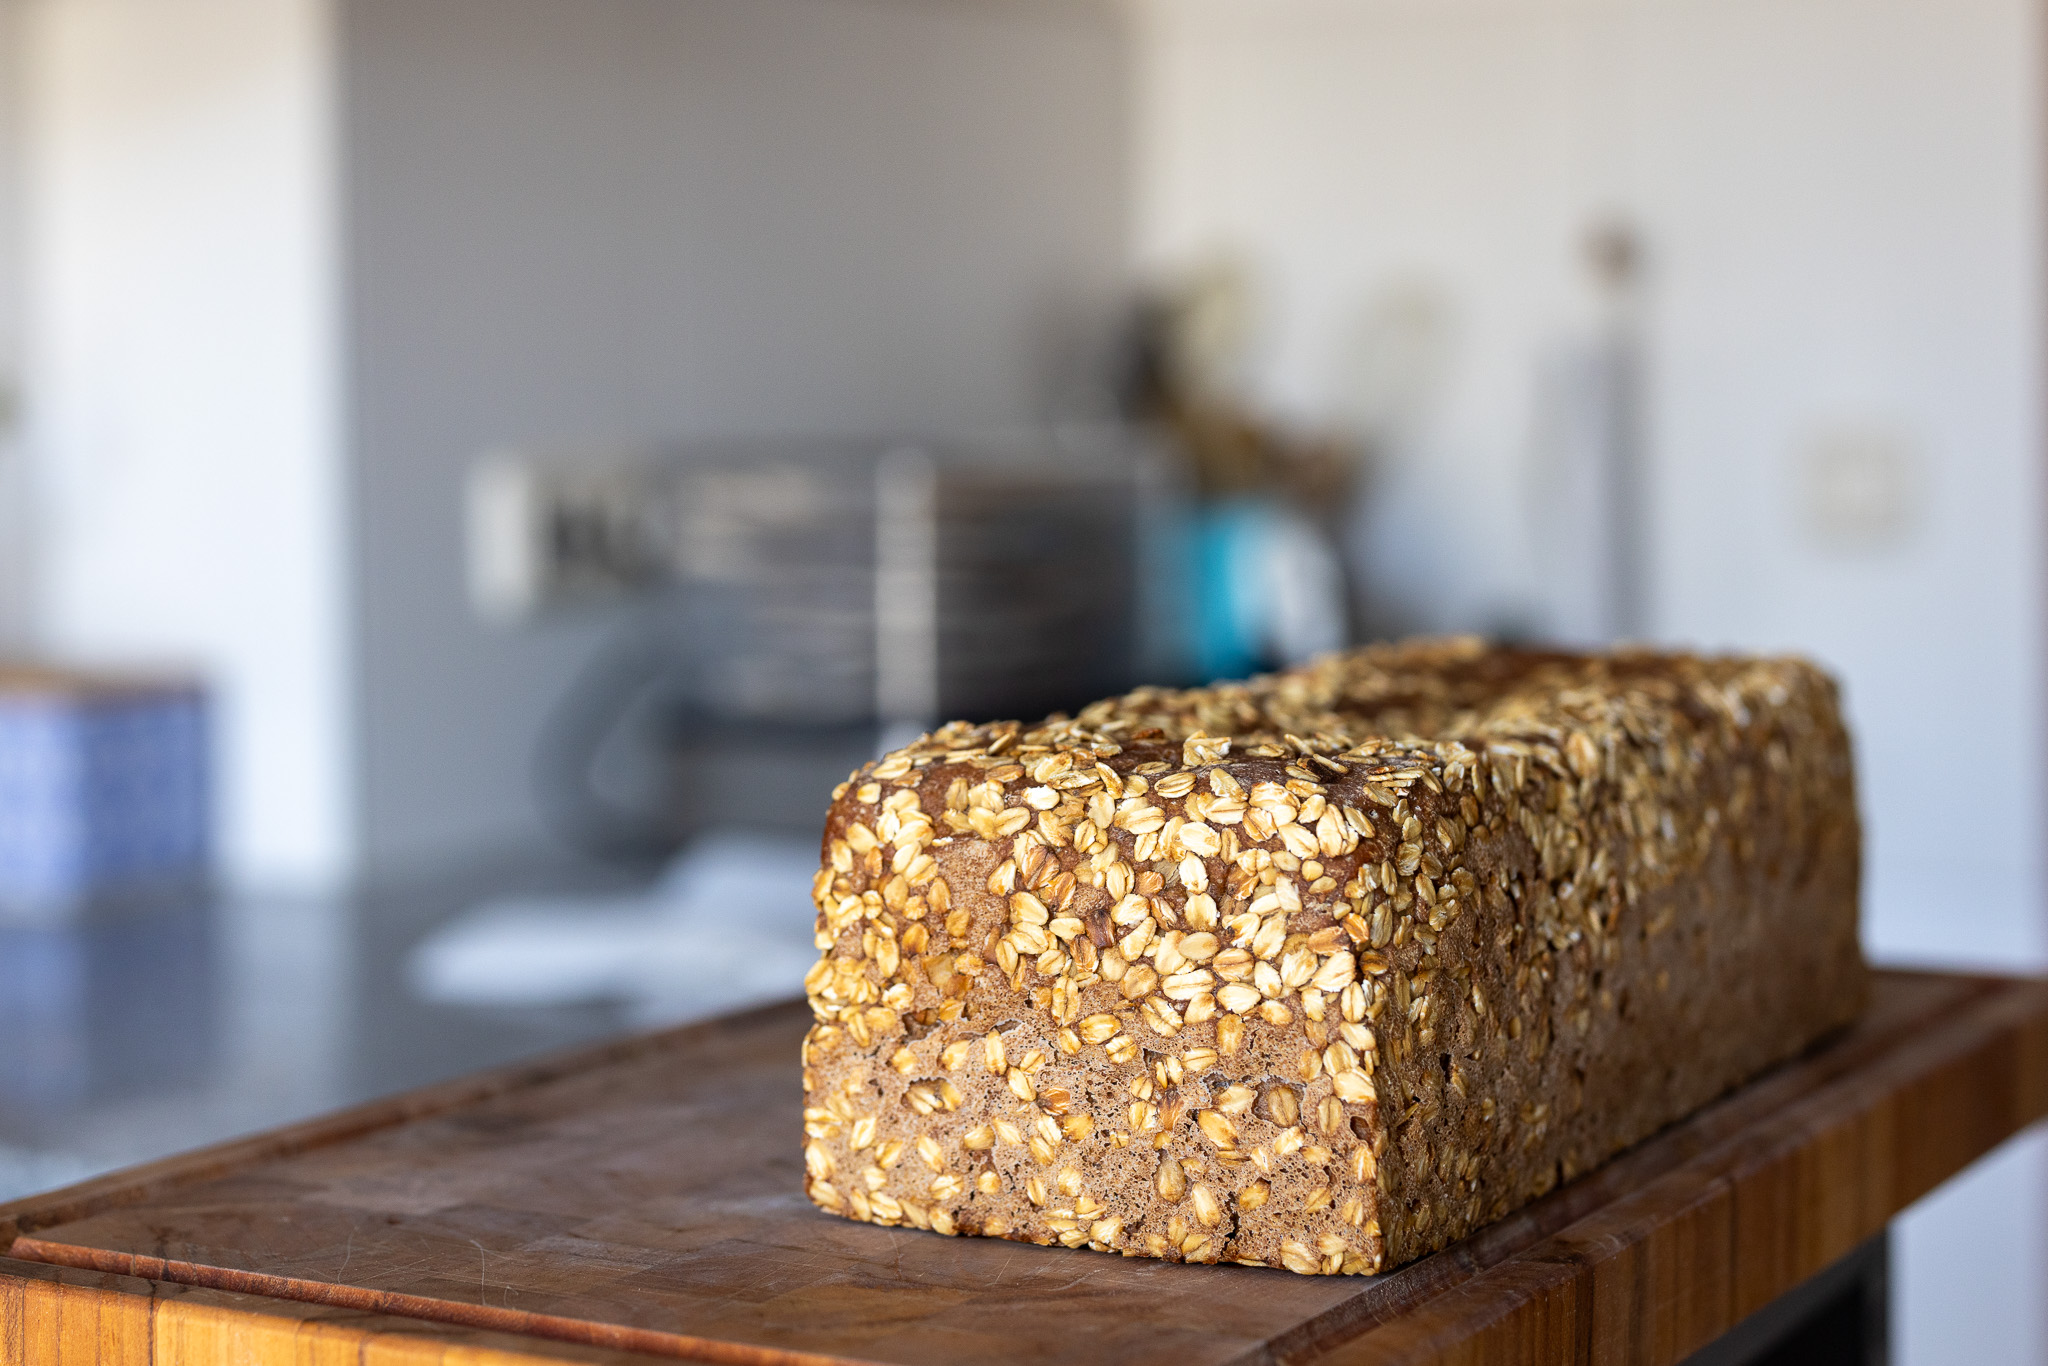
\includegraphics[width=\textwidth]{whole-grain-sandwich-outside}
    \caption{An easy-to-make bread that can be paired with a variety of toppings.}
\end{figure}

\noindent\textbf{Ingredients:}

\begin{center}
\begin{tabular}{|c|l|r|r|}
    \hline
    \textbf{No.} & \textbf{Ingredient} & \textbf{Quantity} & \textbf{Baker's math} \\
    \hline
    1 & Whole-wheat flour, whole-rye flour & 400 g, 400g & 100\% \\
    \hline
    2 & Water, warm & 640 g & 80\% \\
    \hline
    3 & Sourdough starter & 80 g & 10\% \\
    \hline
    4 & Salt & 16 g & 2\% \\
    \hline
\end{tabular}
\end{center}

\noindent\textbf{Instructions:}
\begin{center}
\begin{tabular}{|c|p{12cm}|}
    \hline
    \textbf{Step} & \textbf{Instruction} \\
    \hline
    1 & Mix all the ingredients until there are no chunks of
    flour left. A spatula will make the whole process easier. \\
    \hline
    2 & Wait until the dough has increased by roughly 50~\% in size. \\
    \hline
    3 & Prepare a loaf pan. Use non-stick spray or a good amount of oil. \\
    \hline
    4 & Cover the loaf pan in oats. Shake the oats thoroughly in the loaf
    pan so that they cover the walls. Let the rest of the oats fall out of the
    pan. \\
    \hline
    5 & With a spatula remove the dough from your bulk ferment container and
    cover the whole loaf pan. Gently pat down the dough in your loaf pan so
    that the dough fully covers the pan. \\
    \hline
    4 & Spray some water on the top of your dough, or use a spatula to spread
    water lightly on your dough's surface. Use the remaining oats to cover
    the top of your dough. \\
    \hline
    4 & If you want to bake the bread now, wait 60~minutes letting the dough
    sit on your counter. Alternatively place the dough in your fridge overnight,
    up to a whole week until you are ready to bake. If you let the dough sit
    in the fridge for more than 24~hours I recommend wrapping it in a plastic
    bag so that the surface does not dry out too much. \\
    \hline
\end{tabular}
\end{center}

\noindent\textbf{Baking:}
\begin{center}
\begin{tabular}{|c|p{12cm}|}
    \hline
    \textbf{Step} & \textbf{Instruction} \\
    \hline
    1 & Place the dough into a not preheated oven at 200°C (400°F) \\
    \hline
    2 & Place an inverted oven tray on top of your dough. Not directly
    on the loaf pan, make sure to keep at least 2~cm distance. This
    helps steaming. \\
    \hline
    3 & Wait for at least 45~minutes and let the bread bake. Ideally, take
    a thermometer and measure the core temperature. Especially when fridge
    proofing the dough baking can take longer. Once the dough has
    reached 92°C (197°F) it is ready in theory. However, the top part of the loaf
    might not be properly baked yet. It should have a nice dark color to it
    similar to the the photos. \\
    \hline
    4 & Wait for at least 60~minutes before removing the dough from the loaf pan. \\
    \hline
\end{tabular}
\end{center}

If you feel the final bread is a bit too sour you can toast the slices before
eating them. You can also consider baking your next bread for a longer period.
The heat will evaporate additional acids from the bread and make it taste milder.

\begin{figure}[h]
    \centering
    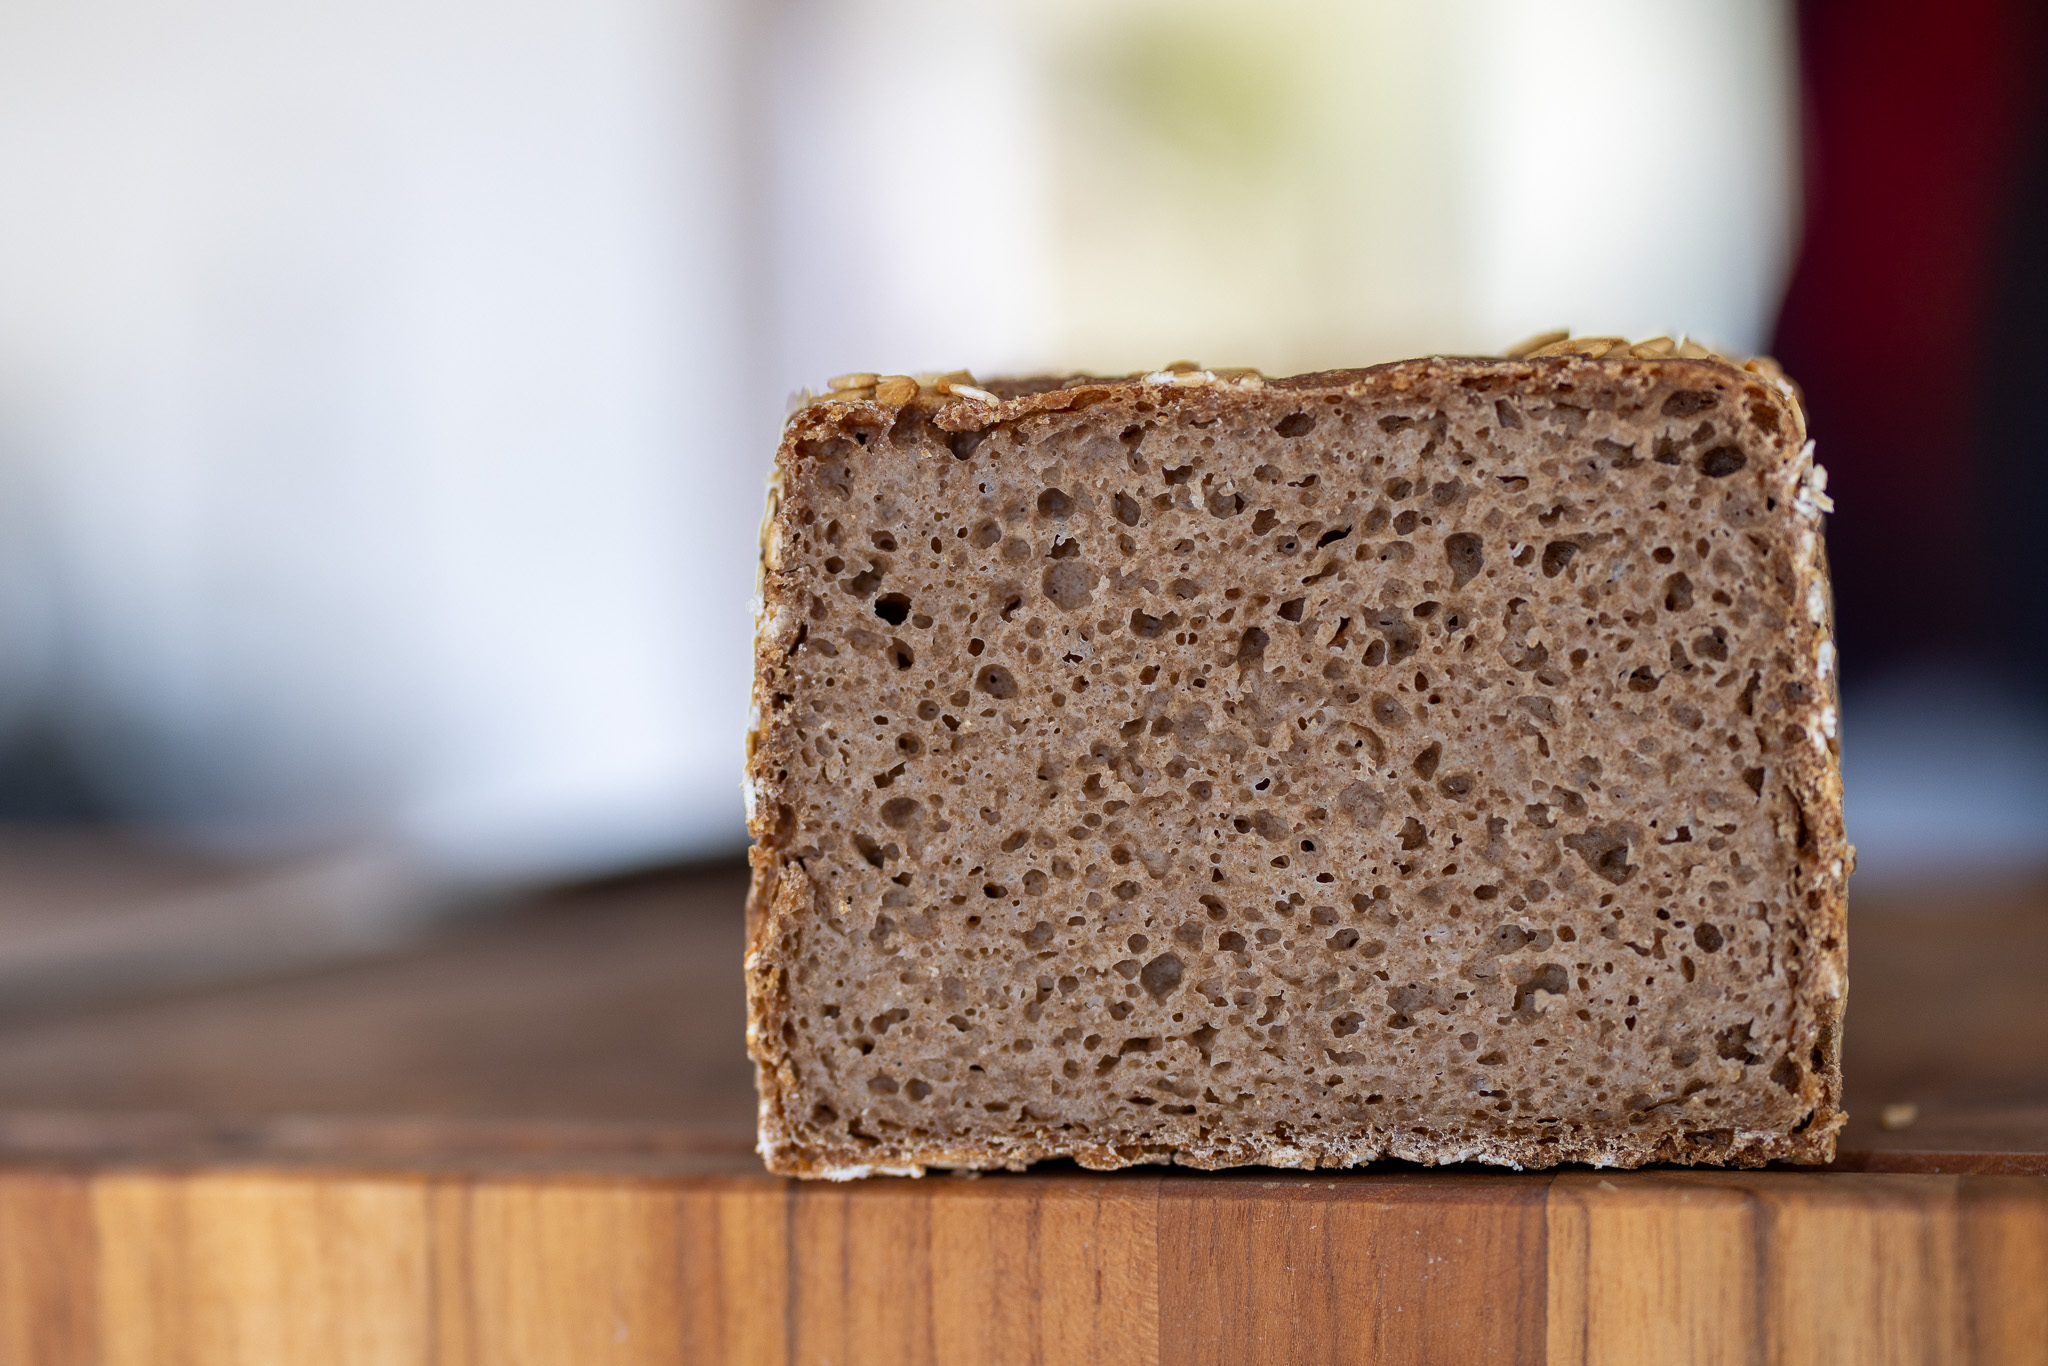
\includegraphics[width=\textwidth]{whole-grain-sandwich-crumb}
    \caption{The bread features a nice soft crumb texture.}
\end{figure}
